\documentclass[12pt]{article}

\newcommand\floor[1]{\lfloor#1\rfloor}
\newcommand\ceil[1]{\lceil#1\rceil}

\usepackage{amsmath}
\usepackage[super]{nth}
\usepackage[utf8]{inputenc}
\usepackage[T1]{fontenc}
\usepackage{textcomp}
\usepackage{gensymb}
\usepackage{graphicx}
\usepackage{changepage}

\pagenumbering{arabic}

\makeatletter
\newcommand*{\rom}[1]{\expandafter\@slowromancap\romannumeral #1@}
\makeatother

\begin{document}

\title{Music Generation in ArtToMusic}
\date{February 22, 2017}
\author{Rafael De Smet}

\maketitle
\tableofcontents

\section{Introduction}

In this paper I will discuss several methods to generate music with software. Analogous to the paper in graphical analysis, I will discuss methods I use in the ArtToMusic project and methods I did not use and compare them to each other. Since music is different for every person, my reasoning can be subjective at times and you may preffer other methods. 

\section{Music generation - a discussion}

\subsection{Rhythm and harmony}

When we listen to music, unconciously we focus on a couple of things to process what we are hearing.

\subsubsection{Rhythm}

One of these things is the rhythm. A very simple way to talk about music and to distinguish between different pieces of music is to say if it is a fast piece or a slow piece. This discussion can be subjective as different people have different notions of speed. Luckily we can objectively determine how fast or slow a piece is, using the BPM (beats per minute).
This tells us how many quarter notes are played in one minute, or how fast/slow the quarter notes are played after each other.
\newline

In the music theory there are a couple of terms to indicate certain intervals of speed, based on the BPM. For example, the term \textit{larghissimo} means that the piece of music has a BPM in the range ]0, 20], which is very slowly. \textit{Moderato} means moderate, so a piece that has a moderate speed usually has a BPM in the range [108, 120]. Most of the popular songs you hear on the radio are \textit{moderato}.

\subsubsection{Melody}

A second crucial part of music is the melody. All melodies of songs are based on the rules of harmony. We can formulate a couple of questions that will help us understand the purpose of harmony, e.g. which notes sound good when played together, and which don't? Which notes make up a chord?
\newline

The notion of chords is very important. A chord is a group of notes played at the same time.
There are major chords, which sound happy, and there are minor chords which sound sad or melancholic. These two types of chords are the most commonly used. There are many other types of chords such as the diminished, the sus4, add9 etc. But for this project I will stick the two most important types and one special chord, the diminished.

\subsection{Chords and progressions}

A crucial element of music is the use of chord progressions. The most common example of this is a twelve bar blues. This type of music is characterised by a strict pattern. Every song that uses a twelve bar blues follows the same chord progression and thus sounds very similar and recongizable.

\begin{figure}[h]
\centering
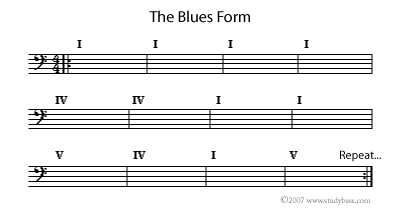
\includegraphics[scale=0.8]{img/the-blues-form}
\caption{Twelve bar blues}
\end{figure}

In figure 1 you can see the structure of a twelve bar blues, very simple yet very recognisable. The roman numbers denote which chord is played, relatively to the key of the song. For example if the piece is in the key of C major, the \rom{1} denotes the first chord of the key, the C chord. The \rom{4} is the fourth chord of the key, the F major. The \rom{5} is the fifth of the key, the G major.
\newline

There are many other kinds of progressions, such as the \rom{1}-\rom{2}-\rom{5}-\rom{1} chord progression, or any other combination. Most popular songs use multiple chord progressions, one for the verse, one for the chorus and so on. It's the concept of combining different chords in one progression that allows us to create new original pieces of music.
\newpage

\subsection{Comparison of music generation techniques}

In this section I will be comparing multiple music generation techniques. I will discuss libraries as well as online applications that have the same goal, creating enjoyable music based on software.

\subsubsection{Beads}
The Beads library, developed by Ollie Bown with the support of the university of Melbourne, is a very handy tool to generate music. Beads uses the concept of unit generators (UGs) as the core of the software. As described by Evan Merz, the author of \textit{Sonifying Processing: The Beads Tutorial} [2], a unit generator is a ``building block of the audio signal''.  One unit generator takes care of one function in the generation of music. 
\newline

A simple example of a unit generator is a guitar player's distortion pedal. The clean signal of his guitar enters the unit generator and a distorted version of the signal is produced. Beads works as a series of unit generators (or guitar pedals). You can plug one UG into another to create a chain of effects, sounds etc... 
\newline

The Beads library has many of these UGs, such as an envelope filter, a gain, a waveplayer, etc. The most important UG is the AudioContext. This is the main UG where every other UG plugs into. Without this there is no music. It doesn't create any sound by itself, it just acts as an interface to the computer's hardware. The audio comes from other UGs.
\newline

Beads has two main ways of creating audio.

\paragraph{Samples}

You can load multiple samples for later use. Once you have found the file and loaded it in via the SamplePlayer, you can use it as any other UG, connect it to the Gain UG to determine the volume or apply multiple effects on it, such as pass it through an EnvelopeFilter, etc.  

\paragraph{Waves}

Another technique is to use audio waves that are generated in real time. The most simple form of audio is a sine wave that produces one tone. Beads has implemented five different kind of waves, each called a Buffer. Each Buffer stores an array of floats in the range [-1,1] that represent the function it is based on. In this list you can see the different buffers and their functions.
\begin{itemize}
\item SINE:  based on the sine function $y(t) = A sin (\omega t + \phi)$
\item SAW: based on the saw function $y(t) = t - \floor{t}$
\item SQUARE: based on the square function $y(t) = sgn(sin(t))$
\item TRIANGLE: based on the triangle function, with range from -1 to 1 and period 2a, $y(t) = \frac{2}{a}(t - a \floor{\frac{t}{a} + \frac{1}{2}}) (-1)^{\floor{\frac{t}{a} + \frac{1}{2}}}$
\item NOISE: based on a random variable to determine each value in the buffer
\end{itemize} 

Every Buffer has other (mathematical) characteristics and thus sounds differently. A sine wave produces a gentle tone, while a saw wave is less enjoyable to listen to.
\newline

Using the Beads library we can create our own music simply by passing the right input parameters to the different UG's to get the desired music.

\subsubsection{Wolfram Tones}

Desgined by the mathematician Stephen Wolfram, WolframTones is an online application to generate music. The user can choose from multiple styles of music and the application generates a new piece of music. The way this works is based on a discovery of Stephen Wolfram himself. In the early 1980s Wolfram was researching ``one-dimensional cellular automata''. He discovered that a set of very simple rules can create a very complex situation. 
\newline

His experiments start with a row of cells, each cell black or white. The set of rules, determined before the execution, decide which colour every cell on the next line will get and so on. Figure 2 shows a possible set of rules. The top row in each box gives one of the possible combinations of colors for a cell and its immediate neighbours. The bottom row then specifies what color the center cell should be on the next step in each of these cases [1]. The rules of figure 2 can be described as follows. A particular cell will be black if either of its neighbours was black on the step before. A cell will be white if both its neighbours were white on the step before.

\begin{figure}[h]
\centering

\includegraphics[]{img/wolframRules}
\caption{Rules for automata}
\end{figure}

\begin{figure}[h]
\centering
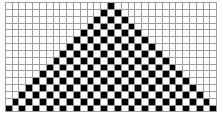
\includegraphics[]{img/wolframResult-15}
\caption{Result automata}
\end{figure}

This gives the result in figure 3. In this case the result is very well structured and organized. Wolfram discovered that there are 256 of these simple sets of rules, based on eight individual rules. Not every one of these 256 sets gives nicely structured results.

\paragraph{Music}

Wolfram used his automata to create music. Let's say we used one of the 256 sets of rules to create a result pattern. We can take a partition through this pattern of 15 cells wide. When we flip this partition on its side we can treat it as a musical score.
Figure 4 shows the partition from a resulting pattern and figure 5 shows it as a musical score.
\newline

 \begin{figure}[h]
\centering
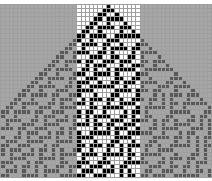
\includegraphics[]{img/wolframMusic1}
\caption{Partition through pattern}
\end{figure}

\begin{figure}[h]
\centering
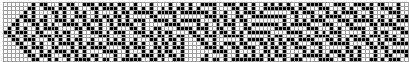
\includegraphics[]{img/wolframMusic2}
\caption{Musical score}
\end{figure}

Now we can assume that time runs across the page from left to right and every black cell represents a note played. Wolfram has developed his own programming language (Wolfram Language [4]) and uses various of his own algorithms to form music out of these cellular automaton patterns.
\newline

The number of rules isn't limited by eight individual rules. We could also determine the color of the next cell by looking at his five upper row neighbours, instead of three. This gives a much bigger number of results (around 4 billion) and much more interesting results to use in the music creation. 

\subsubsection{Genetic algorithms}

Another interesting case to focus on is the use of genetic algorithms to produce music, as explained in the paper by Dragan Matic [2].
\newline

A genetic algorithm (GA) is an algorithm based on the idea of natural selection. The execution of a genetic algorithm starts with an initial population of individuals. During the execution of the algorithm, it will try and find an optimal solution based on predetermined rules. Each indiviual of the population has an attribute 'fitness'. This attribute denotes the quality of each individual of the population.
\newline

This particular GA used in the paper of Dragan Matic uses complete musical compositions as the individuals of the population. A composition is any combination of rhythm and notes, while the concept of good and bad music is represented in the fitness attribute. Because the notion of good and bad music is very subjective and different for each person, Matic uses a reference individual (another composition) for the evaluation of the resulting composition.
\newline

We start with the initial population, containing $n$ individuals. After this, an iterative process begins. The fitness of each individual is calculated in each iteration. Based on the best individual (best fitness), we test if the stop condition is met. This stop condition can be set by the user before execution. If the algorithm decides to stop, the best individual is played.
\newline

If the algorithm continues, we remove two-thirds of the individuals in the population. Mutation operators are applied to the remaining individuals to generate new different individuals. Now the next iteration starts and we calculate the fitness of the new individuals and test if we have found a good composition.

This continues till the stop condition is met.

\paragraph{Determining the fitness}

This GA uses a function to compute the total fitness of an individual based on different criteria. Since there is an extra subjective aspect to music, the end result of the algorithm may suffice to the criteria of the fitness function but still seem a bad choice (bad piece of music) to the listener. 
\newline

Equation 1 gives the total fitness of one individual. $\lambda_i$ represents the weight (influence) of the value $f_i$ to the total fitness and $n$ is the number of criteria [5].

\begin{equation}
f = \sum_{i = 1}^{n}\lambda_i f_i
\end{equation}

There are a couple of ways to go about this. You can say that for different $i$, $f_i$ may be a ratio between the number of tones out of a given tonality and the total number of tones, the ratio between the number of dissonant intervals and all intervals, the ratio between the number of appearances of some pattern in relation to the total number of notes, density of notes, etc [2]. 
\newline

The approach the GA in the paper of Mati\'c uses a more general approach. This means the fitness is calculated from one to another bar, and the total fitness is the sum of those values. Therefore, we have a new definition for $f$.

\begin{equation}
f = \sum_{j = 1}^{k} \sum_{i = 1}^{n}\lambda_{ij} f_i
\end{equation}

where $\lambda_{ij}$ is the weight of value $f_i$ in the $j-th$ bar, $n$ is the total number of criteria and $k$ is the total number of bars.

\paragraph{Comparing with the reference individual}

To know if we have a good piece of music, we must compare it with the predefined reference individual. This similarity is determined based on the "distance" between them. This distance is calculated bar by bar. The distance between individuals, and the appropriate bars of the two individuals in the comparison is based on the number and type of "good" intervals.
\newline

These "good" intervals are predefined, in table 1 at the top of this page, you can see a proposal of these intervals [2]. An interval here means two consecutive notes and their relation to each other, are they in unison, a perfect fourth etc. Based on these values given to every note combination we can compute the fitness level of a bar of music.

\begin{figure}
\begin{tabular}{| c | c | c | c |}
\hline
\textbf{Categories of intervals} & \textbf{Intervals} & \textbf{Values Proposal} \\
\hline
Perfect Consonants & unison, perfect fourth, & 1  \\ 
& perfect fifth, octave & \\
\hline
Imperfect Consonants & minor and major thirds & 2 \\
& and sixths & \\
\hline
Seconds & minor and major seconds & 3 \\
 \hline
Sevenths & minor and major sevenths & 3 \\
\hline
Intervals greater & all intervals greater & 5 \\
than octave & than octave & \\

\hline
\end{tabular}
\end{figure}

\newpage

\subsubsection{Computoser}

Computoser is another web application that generates random music. It is a rule-based, probability-driven algorithm. This means that it composes by following a set of rules and makes decisions between several (musical) alternatives that are based on predefined probabilities.
\newline

Computoser gives probabilities to every type of note interval (analoguos as the intervals in the GA section) and to each note length.
This means that for example a fifth (a distance of five notes in the scale) gets a probability of 25\%. This is a fairly high chance because a fifth is very commonly used in composing.
\newline

Computoser uses seven groups of rules.
\begin{enumerate}
\item Structure of the piece of music 
\item Rhythm; notes must conform to a rhythm scheme
\item Repetition; each component of the piece (a group of notes) is repeated several times for memorability 
\item Variations; slight changes are made to each component to make it more interesting
\item Dissonance and syncopation; unexpected elements in music are what makes it interesting to listen to
\item Endings; there are several ways to end a piece of music
\item Effects; different kind of sounds, such as distortion, tremolo etc
\end{enumerate}

Analogous to the probabilities given to intervals, each of the rules used in the algorithm has a certain percentage that decides which rule to use.
\newline

The components of the Computoser algorithm are called manipulators. They each fill in a part of information of the score. Analogous to the Unit Generators of the Beads library, these work as a chain. Subsequent manipulators depend on previous ones. There are four main manipulators. I pose several questions these manipulators try to solve.

\begin{enumerate}
\item Part configurer: what parts are there in the piece? Is there a bass line, a piano part?
\item Scale configurer: what scale/key is the piece in? The most likely scales are the major and minor scales. Scales like the Dorian are less likely.
\item Meter configurer: what meter is the piece in? 4/4 is the most common meter, but you can have a piece in 6/8, 3/4, etc.
\item Part generator: each part has its own generator and decides for each part what notes to play.
\end{enumerate}
 
The part generator is obviously the most important one of the algorithm, because it decides what notes to play. There are three main aspects to this generator. Again, the decisions are all based on probabilities.

\paragraph{Pitch} Apart from using the probabilities there are a few other constraints used to determine what note to play next. First, there should not be more than two subsequent unstable notes. Unstable notes are notes that are quite dissonant. Secondly, long jumps between notes (more than 7 steps/notes) require a step in the opposition direction. Thirdly, a predefined sequence of notes may be used, if they are from the circle of fifths or part of an extended chord.

\paragraph{Length} Here are the probabilities used as well, but again some other constraints are used. First is the measure size, all measures should have the same length. The second constraint is rhythm. Each measure is either simple (only one down-beat, e.g. 2/4) or compound (more than one down-beat, e.g. 4/4).

\paragraph{Variation} Computoser uses motifs to construct the parts. There are a few simple motifs that we use as a basis. These motifs can undergo several musical variations to create new motifs. A few of these are transposition (all notes go higher or lower within the same scale), inversion (turning the melody 'upside-down'), retrograding (playing the motif backwards), etc.

\section{ArtToMusic's way to generate music}

The most challenging concept of this project is the translation of graphical concepts, things we see on the image, into musical concepts, things we hear. I had to make choices regarding which graphical elements I wanted to translate into music.

\subsection{Rhythm}

I decided to use the edges of objects in the image to determine the rhythm of the music. When you have a picture with a lot of shapes in it, you are likely to get a busier piece of music with complex rhythms. I used edge detection algorithms, discussed in the paper on graphical analysis, to get a representation of the image where only the edges were shown.
Depending on how many edges there are in the image, I randomly generated a BPM. I predefined several ranges based on actual ranges used in musical theory and randomly generated a BPM from these ranges.
If the picture has very few edges, the number would be generated from the \textit{lento} range, [40-60].

\begin{figure}[h]
\centering
\hbox{\hspace{-1.3em}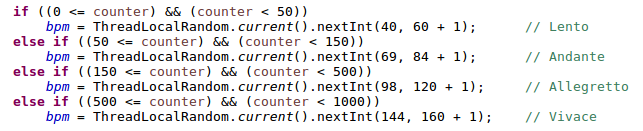
\includegraphics[scale=0.7]{img/bpm_code}}
\caption{Code to determine the BPM}
\end{figure}

\subsection{Melody}

Based on the rules of harmony, the program works with premade chord progressions. These are enumerations of a number of chords in a certain order which creates a melody. For example, the chord progression I-II-V-I is a very commonly used progression. This means we play the first chord of the key we are in, then the second, then the fifth and the first one to end. All of the chords used are major, minor or diminished, based on the rules of harmony.
\newline

Based on how much of certain colors there are in the image we are analysing, we choose a different chord progression to work with. If there is a lot of red in the image, the program chooses the I-II-V-I progression, for instance. Other dominant colors lead to other chord progressions.
\newline

Using the technique of image segmentation, I will determine how many dominant shapes of colors there are. If this number is high, I generate an extra bassline to accompany the main melody. 

\subsubsection{Chord Progressions}

In ArtToMusic I will be using some standard chord progressions and some more unusual ones. There are a few reasons I choose for the use of chord progressions. Firstly, it is the most common way to write music. Secondly, it facilitates the generation of music in code. Several progressions are known to the ArtToMusic program and can be played easily, given the key of the song. 
‌\newline

A few of these standard chord progressions are the following:
\begin{itemize}
\item I-II-V-I: a happy, vibrant sound
\item I-V-VI-IV: a neutral sound
\item I-IV-I-V: a very upbeat sound
\end{itemize} 

To make matters more interesting, I use some famous numbers from mathematics, such as $\pi$, $\phi$ and $e$. These irrational numbers can be seen as a series of digits. These digits can be seen as chords in a progression. For example, the first five digits of $\pi$ are 3, 1, 4, 5, and 1. When we see them as chords we get the following chord progression: III-I-IV-V-I, which seems a very interesting progression.
\newpage

\begin{thebibliography}{1}

\bibitem{beads} Ollie Bown (http://www.beadsproject.net/) 2008

\bibitem{beads_sonifying} Evan X. Merz {\em Sonifying Processing: The Beads Tutorial} 2011

\bibitem{wolfram} Stephen Wolfram {\em A new kind of science} 2002

\bibitem{wolfram language} The Wolfram Language Documentation Center {\em http://reference.wolfram.com/language/guide/LanguageOverview.html}

\bibitem{genetic} Dragan Mati\'c {\em A genetic algorithm for composing music} 2010, Faculty of Natural Sciences, University of Banjaluka, Bosnia and Herzegovina

\bibitem{computoser} Bozhidar Bozhanov {\em Computoser - rule-based, probability-driven algorithmic music composition} 2014,  independent researcher

\end{thebibliography}

\end{document}